\chapter{Information Theoretic Clustering}\label{ch:itm}

Before we start our investigation of semantic segmentation and object class segmentation,
we look into a general purpose clustering algorithm.
%
In clustering, the goal is to divide data points into homogeneous subsets, called
clusters.
Many different formulations of the clustering problem are given in the literature.
%
In the context of this work, clustering plays an important role in many respects:
\begin{itemize}
    \item Clustering, as a purely unsupervised methods is on one end of the
        spectrum of algorithms we investigate.  When using per-image or
        per-pixel supervision as in the later chapters, we can use clustering
        to calibrate our expectation of what semi-supervised and supervised
        algorithms should be able to achieve.

    \item Clustering algorithms build the basis of most superpixel algorithms, and
        better clustering algorithms can lead to better superpixel algorithms.

    \item As many other computer vision algorithms, our segmentation methods
        depends on bag-of-feature representations of segments or images. These
        are built using a vocabulary of visual words that is usually created
        via clustering.
\end{itemize}

So not only is clustering one of the fundamental problems in machine learning, it is also
an important building block for the methods in this work.
%
Most algorithms are based on ad-hoc criteria such as intra-cluster similarity
and inter-cluster dissimilarity.
An alternative approach is to formalize clustering using an information
theoretic framework, where one considers inputs as well as cluster assignments
as random variables.  The goal is then to find an assignment of data points to
clusters that maximizes the mutual information between the assignments and the
observations.

In the following, we rely on a non-parametric estimator of the data entropy to find 
clusterings of maximum mutual information.
%
The use of non-parametric estimates allows a data-driven approach, without 
making strong assumptions on the form of the data distribution.
%
As a consequence, we obtain a very flexible model that, for example, allows 
non-convex clusters.
%
The resulting objective is easy to evaluate, but difficult to optimize
over. We overcome this by proposing an efficient approximate optimization
based on the Euclidean minimum spanning tree algorithm. 
%
Because the estimator and the optimization are both parameter-free, 
the only free parameter of the algorithm is the number of clusters, 
which makes it very easy to use in practice.
%
The contributions of this chapter are:
\begin{itemize}
    \item Proposing the use of a MST-based entropy estimator in information theoretic clustering.
    \item Giving a fast algorithm for a relaxed version of the resulting problem.
    \item Showing the practicality on a number of synthetic and real datasets.
    \item Extending the clustering to data on submanifolds by estimating implicit dimensionality.
\end{itemize}

%CHL: Maybe use this somewhere else, here it sounds redundant.
%While other algorithms have to rely on continuous, gradient-based techniques,
%we can rely on fast, combinatorial optimization.
%
%The run time of the proposed algorithm is dominated by the computation of the Euclidean spanning tree of the
%data, which is possible essentially in $O(n \log(n))$~\cite{dtb2010, eppstein1999spanning}.


\section{Related Work}
The most commonly used clustering algorithm is the $k$-Means algorithm, originally
investigated by \citet{macqueen1967some} and most commonly implemented using
Lloyd's algorithm \citep{macqueen1967some,lloyd1982least}. While
$k$-Means often works well in practice, one of its main drawbacks is the
restriction in cluster shape. 
%
Clusters are given by the Voronoi tessellation of the cluster means and
therefore are always convex.  Another draw-back is the non-determinism of the
procedure, caused by the dependence on random initialization.

Another widely used method is spectral clustering~\citep{shi2000normalized,ng2002spectral}, 
which solves a graph partitioning problem on a similarity
graph constructed from the data. While spectral clustering is much more
flexible than $k$-Means it is quite sensitive to the particular choice of graph
construction and similarity measure. It is also computationally expensive to
compute, because clustering $n$ points requires computing the eigenvalues and
-vectors of an $n\times n$ matrix.

Information theoretic approaches to clustering were first investigated in the
context of document classification. In this setting, training examples are
described by a discrete distribution over words, leading to the task of
\emph{distributional clustering}, which was later related to the Information
Bottleneck method by \citep{slonim1999agglomerative}.
This setting was described in detail by \citep{dhillon2003divisive}. In
distributional clustering, it is assumed that the distribution of the data is
known explicitly (for example as word counts), which is not the case in our
setting.

Later, \citet{banerjee2005clustering} introduced the concept of Bregman
Information, generalizing mutual information of distributions, and showed how
this leads to a natural formulation of several clustering algorithms.
%
\citet{barber2006kernelized} construct a soft clustering by using a parametric model of $p(Y\given X)$.
%
The framework of mutual information based clustering was extended to
non-parametric entropy estimates by \citet{faivishevsky2010nonparametric}.
They use a nearest neighbor based estimator of the mutual information, called
MeanNN, that takes into account all possible neighborhoods, therefore combining
global and local influences. The approximate mutual information is maximized
using local search over labels.
%discuss this later in detail
%While optimizing MeanNN allows for non-convex
%clusters, in practice the result is strongly biased towards compact, convex
%regions. This can be explained by a close connections of MeanNN to $k$-Means,
%see Section~\ref{discussion} for an in-depth discussion.

Clustering algorithms based on minimum spanning trees have been studied early
on in the statistics community, due to their efficiency.  One of the earliest
methods is single-link agglomerative clustering~\citep{gower1969minimum}.
Single-link agglomerative clustering can be understood as a minimum spanning
tree-based approach in which the largest edge is removed until the desired
number of components is reached.  \citet{zahn1971graph} refines this criterion
by cutting edges that are longer than other edges in the vicinity. This
approach requires tuning several constants by hand. More recently,
\citet{grygorash2006minimum} proposed a hierarchical MST-based clustering
approach that iteratively cuts edges, merges points in the resulting
components, and rebuilds the spanning tree.
We limit our discussion to the most widely used algorithm from~\citep{gower1969minimum}.
%
\section{Clustering Using Non-Parametric Entropy Estimates}
In general, the goal of clustering can be formulated as follows: 
given a finite collection of samples $\mathbf{x} = (x_1, \dotsc, x_n)$, we want to 
assign cluster-memberships $\mathbf{y} = (y_1, \dotsc, y_n ), y_i \in \{1, \dotsc k\}$ to these samples.
%
We adopt the viewpoint of information theoretic clustering of \citet{gokcay2002information}, 
where the $x_i$ are considered i.i.d{.} samples from a distribution $p(X)$, and the 
$y_i$ are found such that the mutual information $I(X, Y)$ between the distribution $p(X)$ and the
assigned labels $p(Y)$ is maximized.
We can rewrite this objective as 
\begin{align}
         I(X, Y)
        &= D_{\text{KL}}(p(X, Y) \parallel p(X) p(Y)) = H(X) - \sum_{y=1}^k p(Y{=}y) H(X \given Y {=} y)
\end{align}
where
\begin{itemize}
\item $\displaystyle D_\text{KL}\, = \int_\mathcal{X} p(X) \ln\left(\frac{p(X)}{q(X)}\right)\,dX$ is the Kullback-Leibler divergence,
\item $\displaystyle H(X)\, = \int_\mathcal{X} p(X) \ln(p(X))\,dX$ is the differential entropy, and
\item $\displaystyle H(X \given Y{=}y)\, = \int_\mathcal{X} p(X \given Y {=}y) \ln(p(X \given Y {=} y))\,dX$ is the conditional differential entropy.
    \end{itemize}
Expressing the mutual information in terms of the entropy is convenient, since
the objective then decomposes over the values of $Y$. 
%
Additionally, $H(X)$ is independent of the distribution of $Y$ and therefore
does not influence the search over $\mathbf{y}$.

Because we are given only a finite sample from $p(X)$, there is no way to
exactly compute $I(X, Y)$, and this is still true if we fix a set of cluster
indicators $y_i$.
%
Possible ways to overcome this are:
\begin{enumerate}
    \item Fit a parametric model $\hat{p}(X, Y \given \theta)$ to the observations.
    \item Use a non-parametric model $\hat{x}$ to approximate $p(X, Y)$. 
    \item Estimate $H(X \given Y)$ directly using a non-parametric estimate.
\end{enumerate}
We choose the third option, as it is the most flexible while avoiding
the curse of dimensionality that comes with using non-parametric density estimates.

Let $\mathbf{x}_y$ be the set of $x_i$ with label $y$. 
Given a non-parametric density estimator $H_\text{est}$
we have $H_{est}(\mathbf{x}_y) \approx H(X \given Y {=} y)$, leading to the clustering problem
\begin{align}\label{eq:general_objective}
     \max_{\mathbf{y}}\quad - \sum_{y=1}^k p(Y{=}y) H_\text{est}(\mathbf{x}_y),
\end{align}
where the probability $p(Y{=}y)$ is given by the empirical frequency of $y$: 
\[
    p(Y\,{=}\,y)= \frac{n_y}{n} \text{,\quad with\quad} n_y = |\{i \mid y_i = y \}|.
\]

\subsection{Minimum Spanning Tree Based Entropy Estimation}
From now on, we assume that $\mathcal{X}=\mathbb{R}^d$ and $p(X)$ is
absolute continuous.
This setting allows the use of the non-parametric entropy estimate of
\citet{hero1999asymptotic}, that constructs a minimum spanning tree of the data
and obtains an estimate of the data entropy from the logarithm of the length of
the spanning tree.
%
More precisely, the entropy estimate of a dataset $\mathbf{x} = (x_1, \dotsc, x_n)$ is given by
\begin{align}\label{eq:hmst}
    H_{mst}(\mathbf{x}) = d \log(L) - (d-1) \log(n) + \log(\beta_d)
\end{align}
where $L$ is the length of a minimum spanning tree $T(\mathbf{x})$ of $\mathbf{x}$ and $\beta_d$ is an
unknown, but data-independent constant.
The estimator $H_{mst}$ is consistent in the sense that $H_{mst}(\mathbf{x}) \rightarrow H(X)$
for $n \rightarrow \infty$~\citep{hero1999asymptotic}.
Using \Eqref{hmst} as a non-parametric entropy estimate in \Eqref{general_objective} yields
the problem to maximize $\hat{I}(\mathbf{x}, \mathbf{y})$ with
\begin{align}\label{eq:objective}
     \hat{I}(\mathbf{x}, \mathbf{y}) := & -\sum_{y=0}^k p(y) \Bigl[ d \log(L_y) - (d-1) \log{n_y} \Bigr] + C,\\
    = & - \sum_{y=0}^k p(y) \Bigl[ d \log(\bar{L}_y  ) + \log{n_y} \Bigr] + C'\\
    = & - d \sum_{y=0}^k p(y) \log(\bar{L}_y  ) - \sum_{y=0}^k p(y) \log{p(y) + C''} \label{eq:objective_simplified}
\end{align}
where $n_y$ is the cardinality of $\mathbf{x}_y$, $L_y$ is the length of the
minimum spanning tree $T(\mathbf{x}_y)$ and $C$, $C'$ and $C''$ are constants independent of
$\mathbf{y}$.  We defined $\bar{L}_y := \frac{L_y}{n_y}$, the mean edge length
per node in $T(\mathbf{x}_y)$.

\Eqref{objective_simplified} has a natural interpretation: The first term
penalizes long spanning trees, weighted by the size of the cluster. The second
term favors a high entropy of $p(y)$, leading to balanced clusters. Note that
there is a natural trade-off between enforcing intra-cluster similarity,
expressed through $L$ and the balancing of cluster sizes. This trade-off is
similar to formulating an objective in terms of a loss and a regularizer. In
contrast to the ``loss+regularizer'' setup, where the trade-off needs to be
specified by the user, the trade-off in \Eqref{objective_simplified}, given by
the factor $d$, is a direct consequence of the entropy estimator.

The reliance on the dimensionality of the ambient space $\mathbb{R}^d$ can be
seen as the requirement that $d$ is actually the intrinsic dimensionality of
the data.
This requirement is made explicit in our assumptions of an absolute continuous
data density: If the support of $p(X)$ was a lower-dimensional sub-manifold of
$\mathbb{R}^d$, $p(X)$ could not be absolute continuous.

\begin{algorithm}[t]
\begin{algorithmic}\label{overall}
    \Require Points $\mathbf{x}$, desired number of clusters $k$.
    \Ensure Clustering $\mathbf{y}$ of $\mathbf{x}$
    \State $G \leftarrow T(\mathbf{x})$
    \For{$i=0,\dotsc,k-1$}
        \For{$G_j, j=0,\dotsc, i$ connected components of $G$}
            \State $e_j \leftarrow \text{SplitCluster}(G_j)$
        \EndFor
        \State $l \leftarrow \displaystyle \argmax_j\  \hat{I}(G_j \setminus e_j)$
        \State $G \leftarrow G \setminus e_l$
    \EndFor
    \Statex
    \Function{SplitCluster}{$G$}
        %\Require Euclidean minimum spanning tree $T$, dimension $d$
        %\Ensure $e^* = \displaystyle \argmax_{e\in E(T)} \ \hat{I}(G \setminus e )$
        \State Pick arbitrary root $x_0$ of $G$.
        \For{node $x$ starting from leaves}
            \State $w_x \leftarrow \displaystyle \sum_{c \in \text{children}(x)} w_c + d(x, c)$
            \State $n_x \leftarrow \displaystyle 1 + \sum_{c \in \text{children}(x)} n_c$
        \EndFor
        \For{node $x$}
        \State $w'_x \leftarrow w_{\text{root}} - w_x$
        \EndFor
        \For{$e \in E(G), e=(c, p)$, $p$ parent of $c$}
            \State $v_c \leftarrow w'_p + w_p - w_c - d(p,c)$
            \State $m_c \leftarrow n - n_c$
            \State objective$(e) \leftarrow d m_c \ln(m_c) - (d-1) m_c \ln(v_c) + d n_c \ln(n_c) - (d-1) n_c \ln (w_c)$
        \EndFor
        \State $e^* \leftarrow \displaystyle \argmax_{e \in E(G)} \ \text{objective}(e)$
        
    \EndFunction
\end{algorithmic}
\caption{Information Theoretic MST-based Clustering}

\end{algorithm}

\subsection{Finding Euclidean Minimum Spanning Tree Clusterings}
The objective given by \Eqref{objective} is a non-linear combinatorial
optimization problem. It has two properties that make it hard to optimize:
\begin{enumerate}
    \item The objective depends in a non-linear way on $L_y$.
        This makes linear programming techniques, that proved successful for
        other combinatorial task, not directly applicable.
    \item $L_y$ is defined in terms of minimum spanning trees. This set is hard
        to characterize, as changing the cluster membership of a single node may change
        the two minimum spanning trees involved completely.
\end{enumerate}

\begin{figure}
\centering
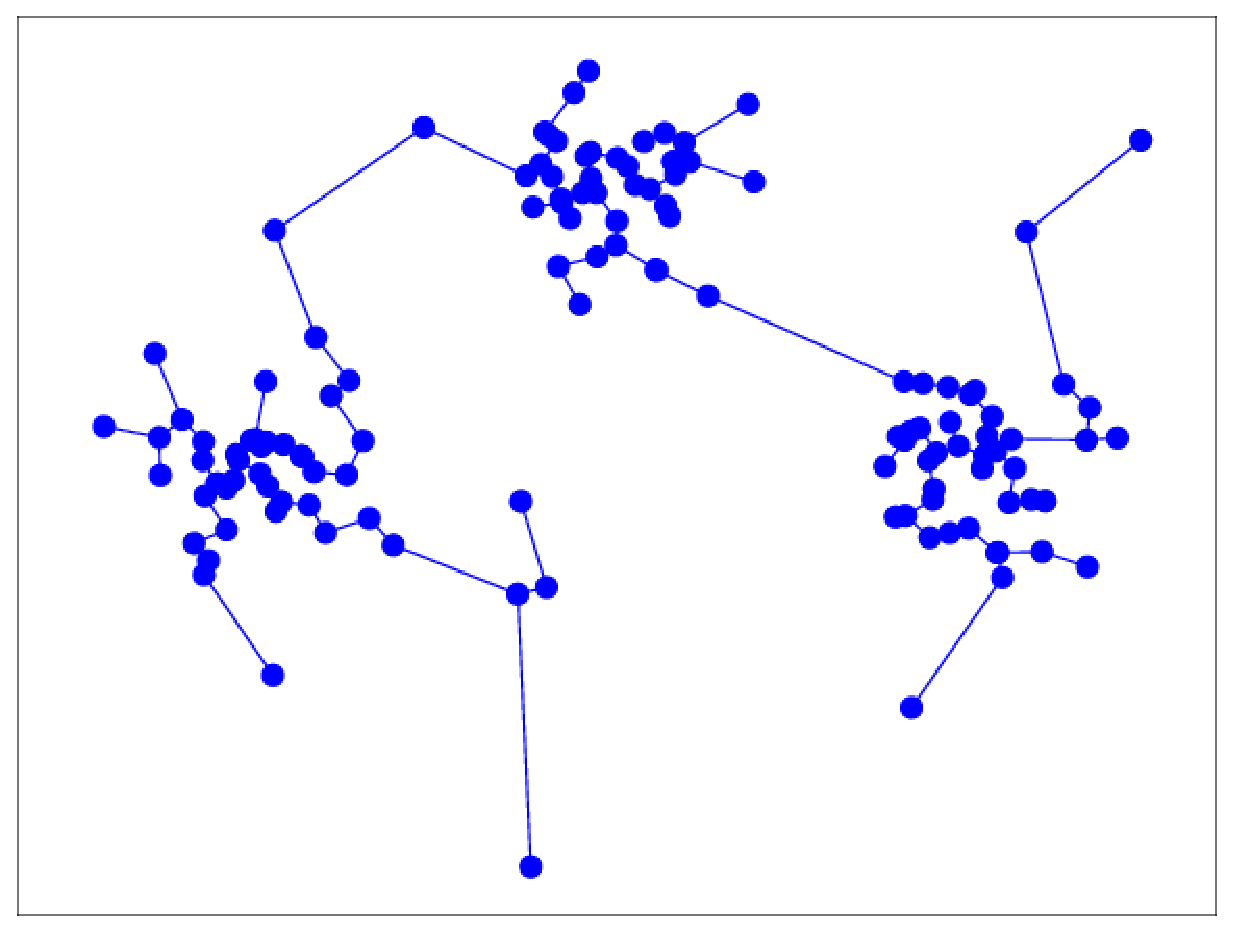
\includegraphics[width=.32\textwidth]{illustration_left}
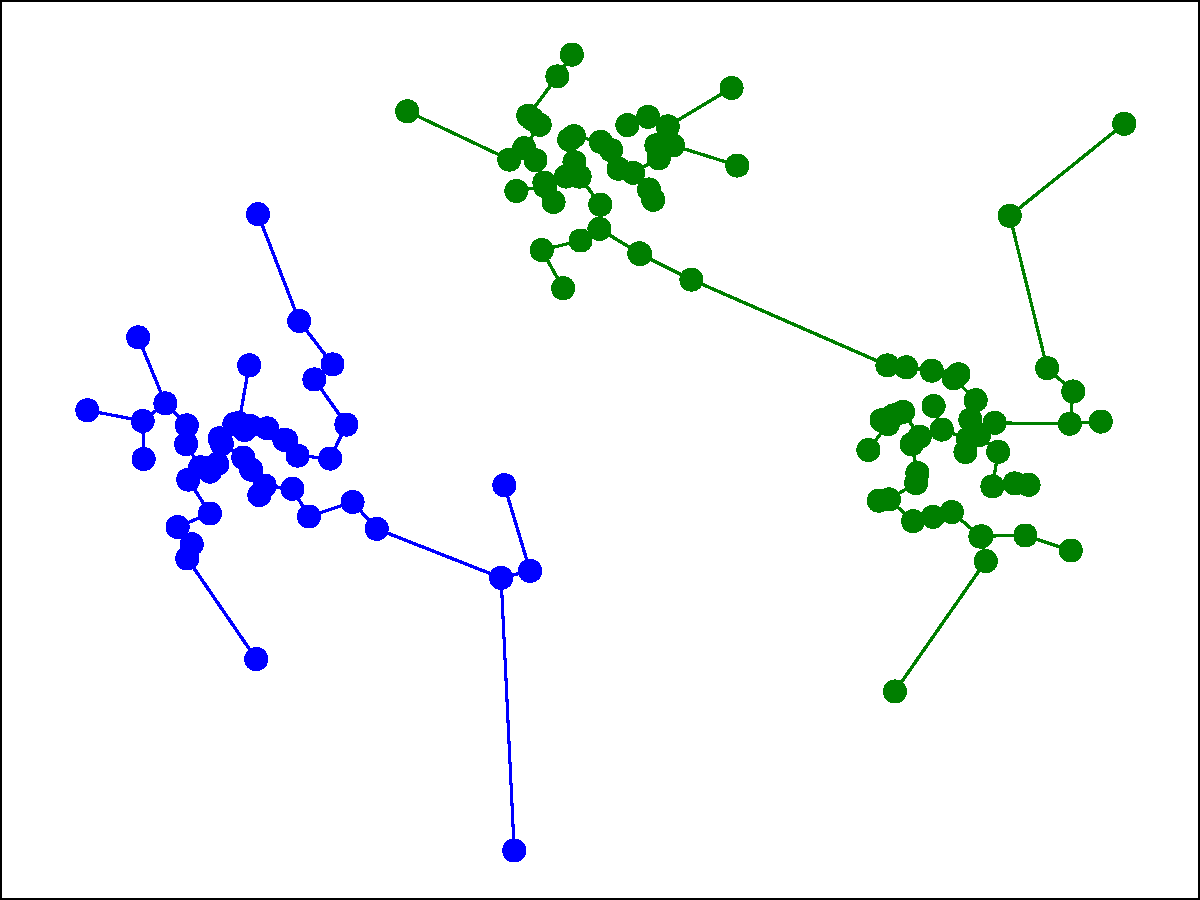
\includegraphics[width=.32\textwidth]{illustration_center}
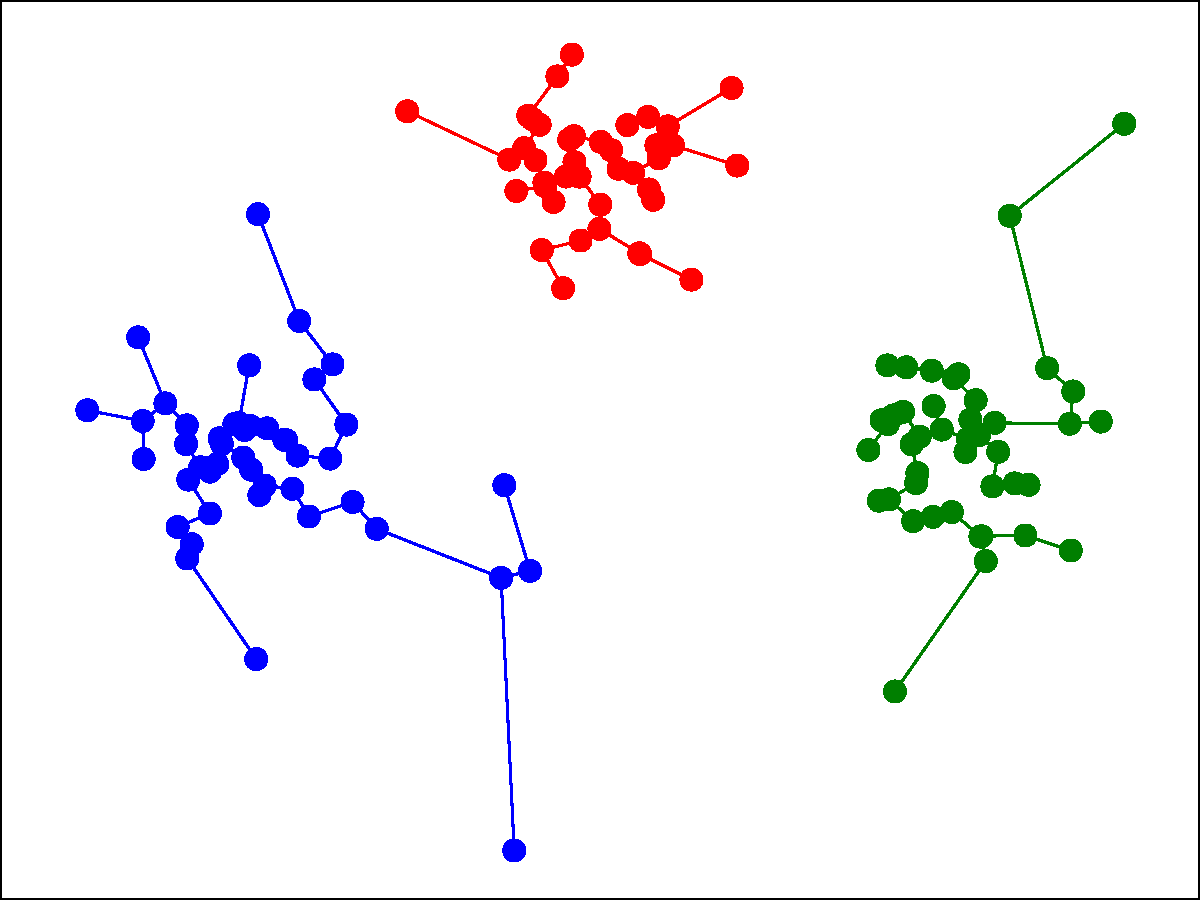
\includegraphics[width=.32\textwidth]{illustration_right}
\caption{Illustration of the optimization algorithm for $k=3$ on synthetic
dataset. \emph{Left}: Euclidean minimum spanning tree of the data.
\emph{Center}: The edge that yields the best two-cluster partition in terms of
\Eqref{objective} was removed, yielding two connected components. \emph{Right}:
Another edge from the forest was removed, resulting in the desired number of
three components. Note that the edge that are removed are not the longest edges
but form a trade-off between edge length and cluster size.}
\label{fig:illustration}
\end{figure}

For the above reasons, we propose a simple procedure to approximately solve
\Eqref{objective}.
%filler removed Let us first fix some notation.
Consider a graph $G$ with nodes $\mathbf{x}$ and edge weights given by the
Euclidean distances between points.  The connected components of $G$ induce a
clustering $\mathbf{y}(G)$ of $\mathbf{x}$, by assigning $x_i$ and $x_j$ the
same cluster if and only if they are in the same connected component of $G$.
Define
\begin{align}\label{eq:graphobjective}
\hat{I}(G) := - \sum_{y=0}^k p(y) \Bigl[ d \log(L_{G,y}) - (d-1) \log{n_y} \Bigr],
\end{align}
where $y$ enumerates the connected components $G_0, \dotsc, G_k$ of $G$, $n_y =
|V(G_y)|$ is the number of nodes in $G_y$ and $L_{G,y} = \sum_{e \in E(G_y)}
w(e)$ is the sum of the weights of all edges in the connected component $G_y$.
%
Then $\hat{I}(G) \geq \hat{I}(\mathbf{y}(G))$, by the definition of
the minimum spanning tree, and equality holds if and only if $G_y$ is the
minimum spanning tree of its nodes for all $y$.
%
We try to find a graph $G$ with $k$ components, such that $\hat{I}(G)$ is maximal. We can restrict
ourself to optimizing over the set $\mathcal{F}$ of forests over $\mathbf{x}$ with $k$ components,
as adding edges inside connected components only decrease the objective.
Thus we can formulate the clustering problem equivalently as
\begin{equation}
    \max_{G \in \mathcal{F}} \hat{I}(G).
\end{equation}


Optimization over forests remains hard, and we further restrict ourself to
solutions of the form $\mathcal{G} := \{ F \in \mathcal{F} \mid F \text{\ subgraph of\
} T(\mathbf{x}) \}$ for a given minimum spanning tree $T(\mathbf{x})$, leading to
the problem $\displaystyle \max_{G \in \mathcal{G}} \hat{I}(G)$.  This restriction allows for
a very fast, combinatorial optimization procedure.


For the two class case, optimization of the above objective can be solved
exactly and efficiently by searching over all of $\mathcal{G}$.
This amounts to searching for the edge $e$ that maximizes $\hat{I}(T(\mathbf{x})
\setminus e)$. The naive algorithm that computes the objective for each edge
separately has run time that is quadratic in the number of data points.  To
improve upon this, we use a dynamic programming approach as described in
Algorithm~1, in function SplitCluster, which has only linear
complexity. Using this algorithm, run time in the two cluster case is dominated
by computing $T(\mathbf{x})$.
%
We extend this algorithm to the case of more than two clusters in a greedy way:
Starting with the full spanning tree of $\mathbf{x}$, we remove the edge
yielding the lowest value of \Eqref{graphobjective} until the number of
components equals the number of desired clusters. The overall procedure is
summarized in Algorithm~1, an illustration can be found in
\Figref{illustration}. We refer to Algorithm~1 as \emph{Information
Theoretic MST-based (ITM) clustering}.

We use Prim's algorithm combined with a ball tree data structure for distance
queries to compute the minimum spanning tree of the data.
While this procedure has no strong runtime guarantees, we found this faster
in practice than specialized algorithms for euclidean minimum spanning trees, 
which achieve a better theoretical runtime of $O(n \log(n) \alpha(n))$ \citep{dtb2010}. Here
$\alpha$ is the inverse of the Ackerman function. The dynamic programming solution of
Algorithm~1 has a run time of $O(n)$ per removed edge, leading to an overall
run time of $O(n \log(n) \alpha(n)+ nk)$. The $O(nk)$ comes from a worst case
scenario, in which each step in the hierarchical clustering procedure only
splits off a constant number of points. In a more realistic setting, we expect
that the individual clusters are much smaller than the original dataset. In
this case, the $O(nk)$ factor would improve to $O(n\log(k))$.

\subsection{Estimating Intrinsic Dimensionality}
While assuming totally continuous densities is very natural from a theoretical
point of view, it can be a hindrance in practical applications.  Often, the
data is assumed to lie on a submanifold, embedded in a
higher-dimensional space. In this case, the density is not totally continuous,
and the dimensionality of the data can not be taken as the dimensionality of
the embedding space.

A particularly drastic example is the case of the dataset having less samples
than features. In this case, the data clearly lies even on a linear subspace
of the input space, and the dimensionality of the input space does not
accurately reflect the intrinsic dimensionality of the data.
We use the estimate analyzed in \citet{massoud2007manifold}.
In their method, for each data point $x$, a local estimate $\hat{d}(x)$ of the
dimensionality at $x$ is computed as
\begin{equation}
    \hat{d}(x) = \frac{\ln 2}{\ln\left(r_k(x) / r_{\lfloor k /2 \rfloor}(x)\right)}.
\end{equation}
Here $k$ is a fixed integer and $r_k(x)$ is the distance of $x$ from its $k$th neighbor.
We follow \citet{massoud2007manifold} and set $k =\lceil 2 \ln n\rceil$.
The final estimate $\hat{d}$ is then computed by averaging the estimates over all $x$
\begin{equation}
    \hat{d} = \frac{1}{n}\sum_{x \in X} \min\left(\hat{d}(x),\ d\right).
\end{equation}
We compute the density estimate once, prior to clustering, and then plug the
estimate $\hat{d}$ into \eqref{graphobjective} in place of $d$.
We found this estimate to work robustly and give sensible results for all
datasets we investigated. As we already used a ball-tree data structure to
build the minimum spanning trees, we can reuse this structure to compute $r_k$.
Consequently, estimating the dimensionality resulted only in little
computational overhead.

\begin{figure}[t]
\centering
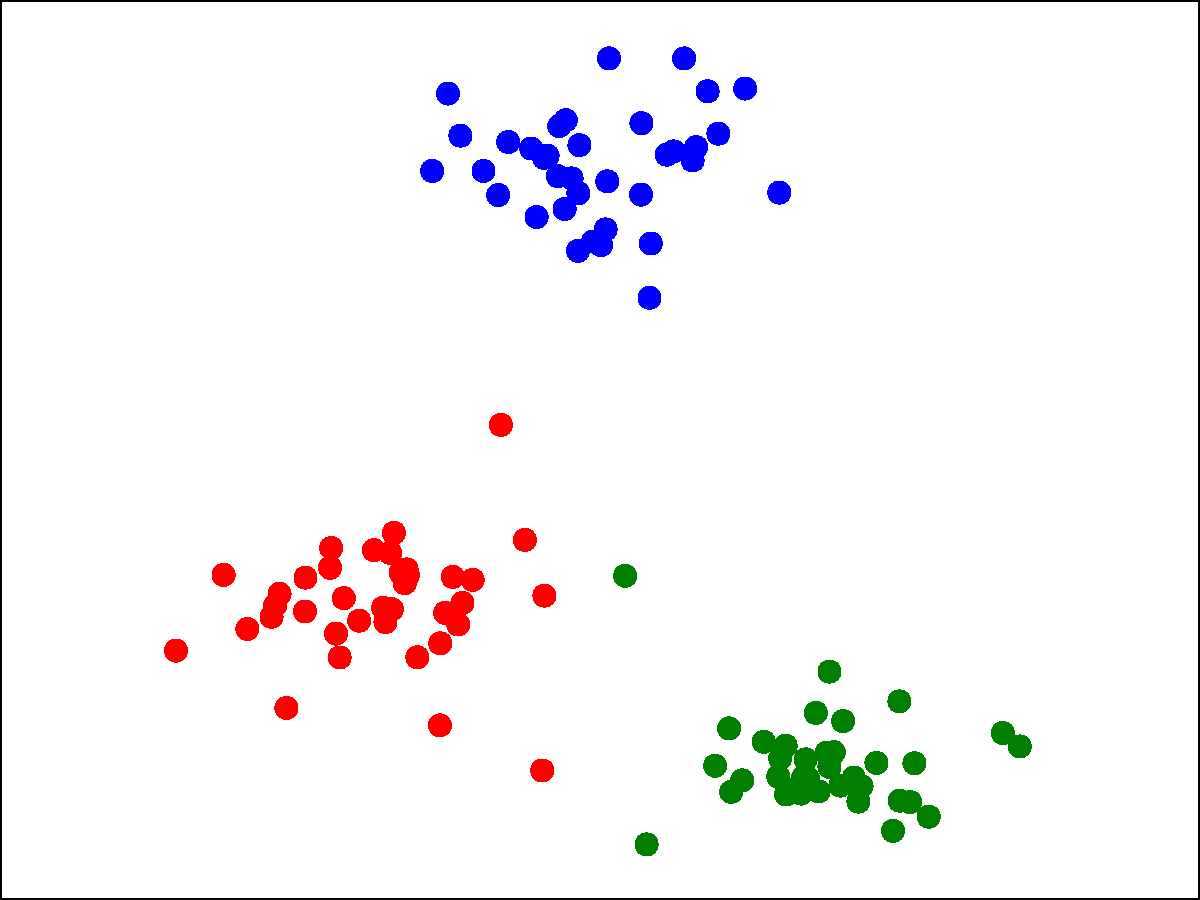
\includegraphics[width=.24\textwidth]{qualitative_blobs_km}
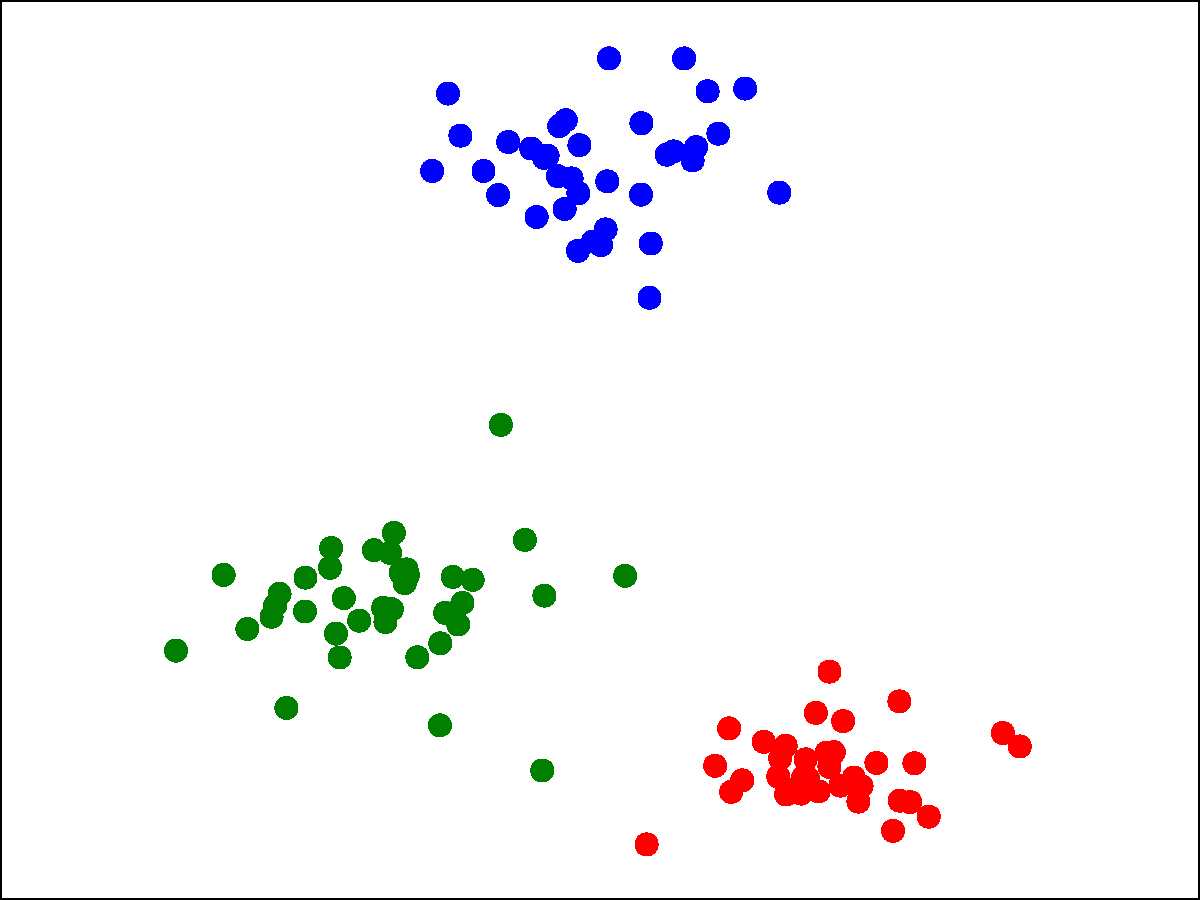
\includegraphics[width=.24\textwidth]{qualitative_blobs_mean_nn}
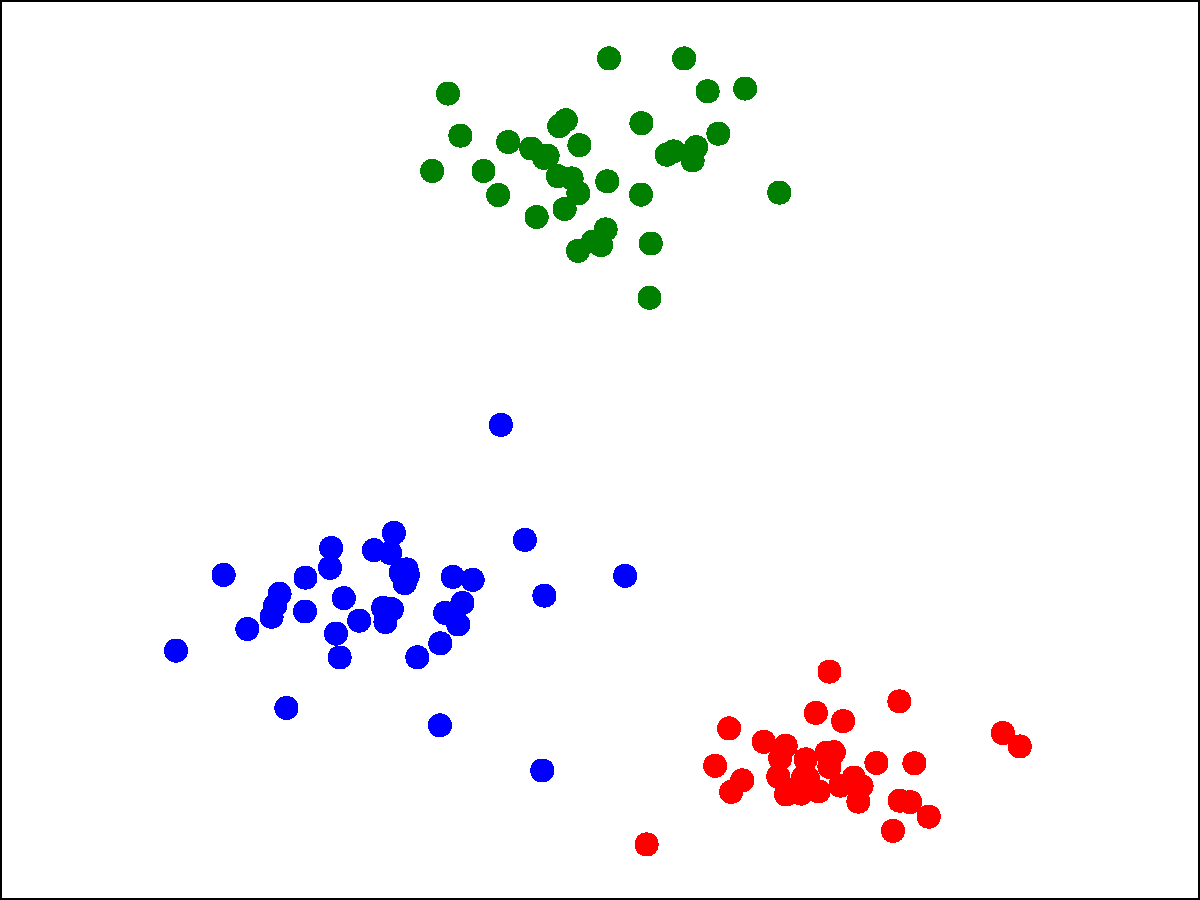
\includegraphics[width=.24\textwidth]{qualitative_blobs_aggl}
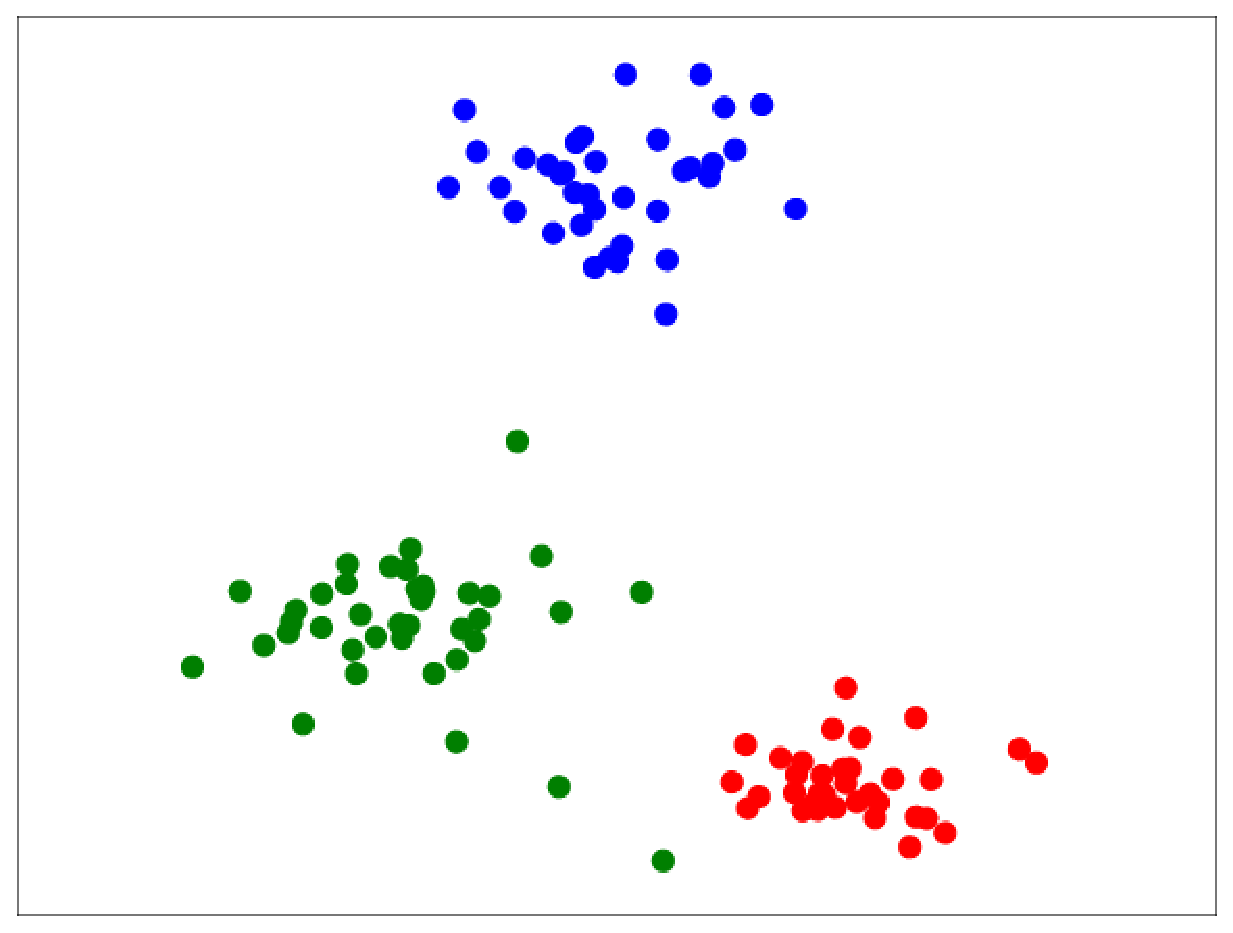
\includegraphics[width=.24\textwidth]{qualitative_blobs_mst} \\ 

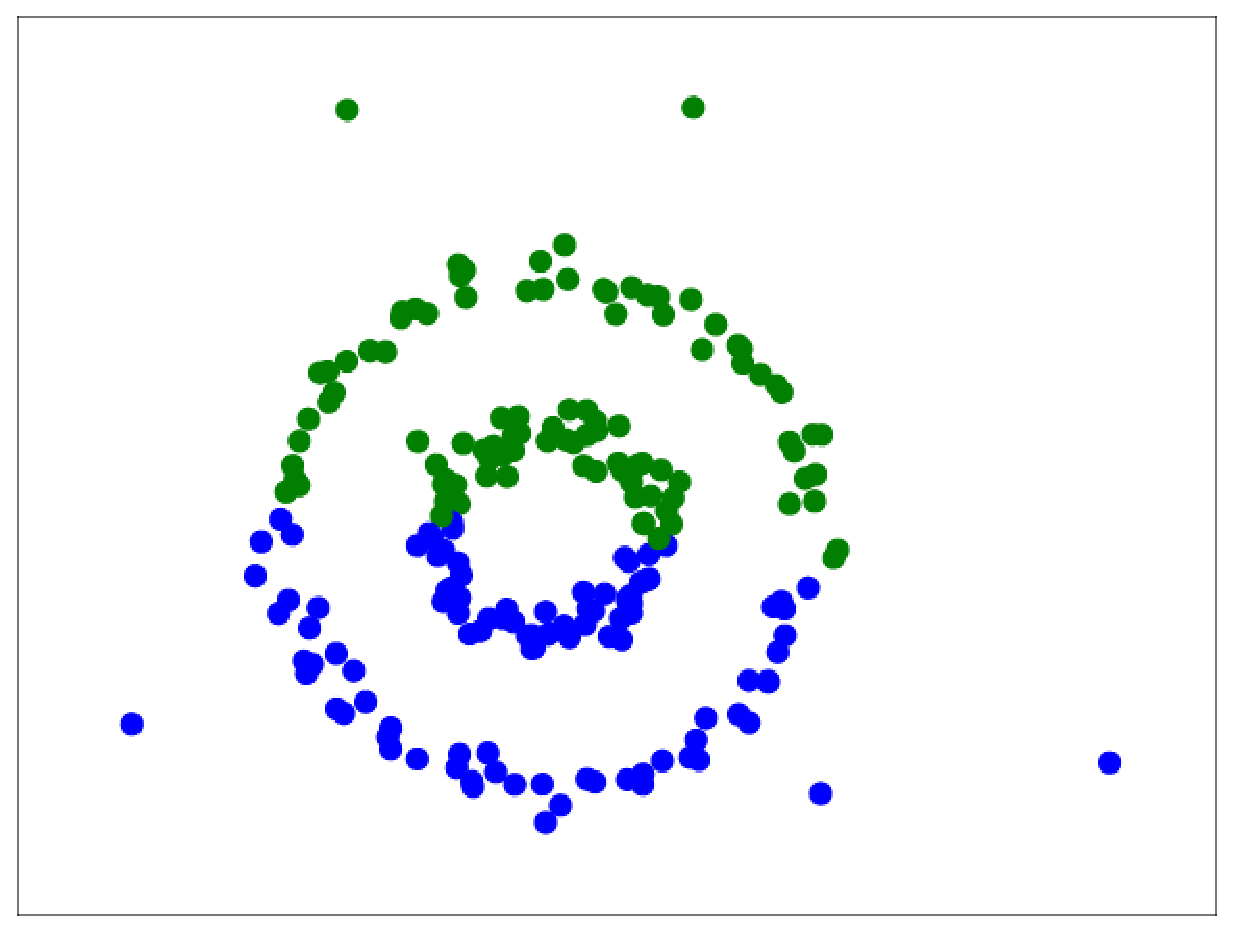
\includegraphics[width=.24\textwidth]{qualitative_circles_km}
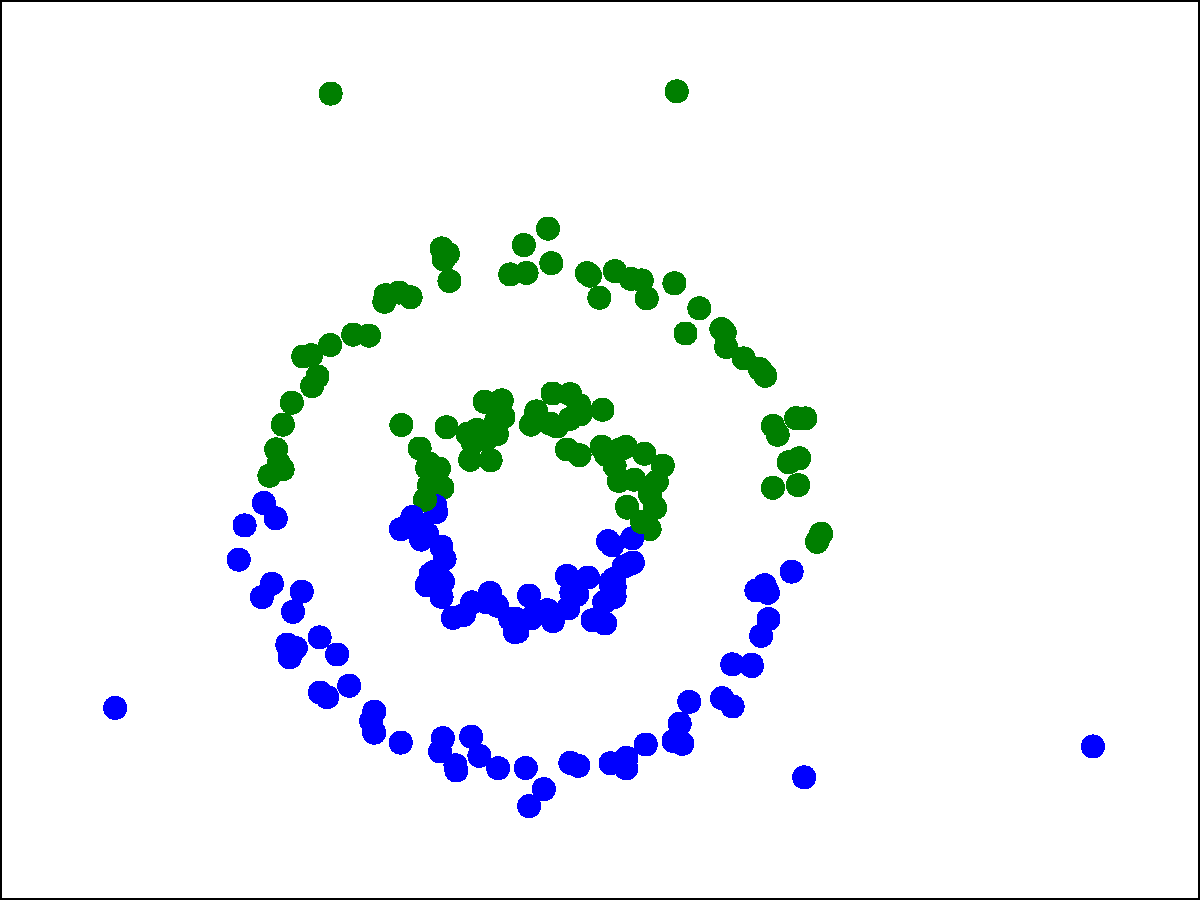
\includegraphics[width=.24\textwidth]{qualitative_circles_mean_nn}
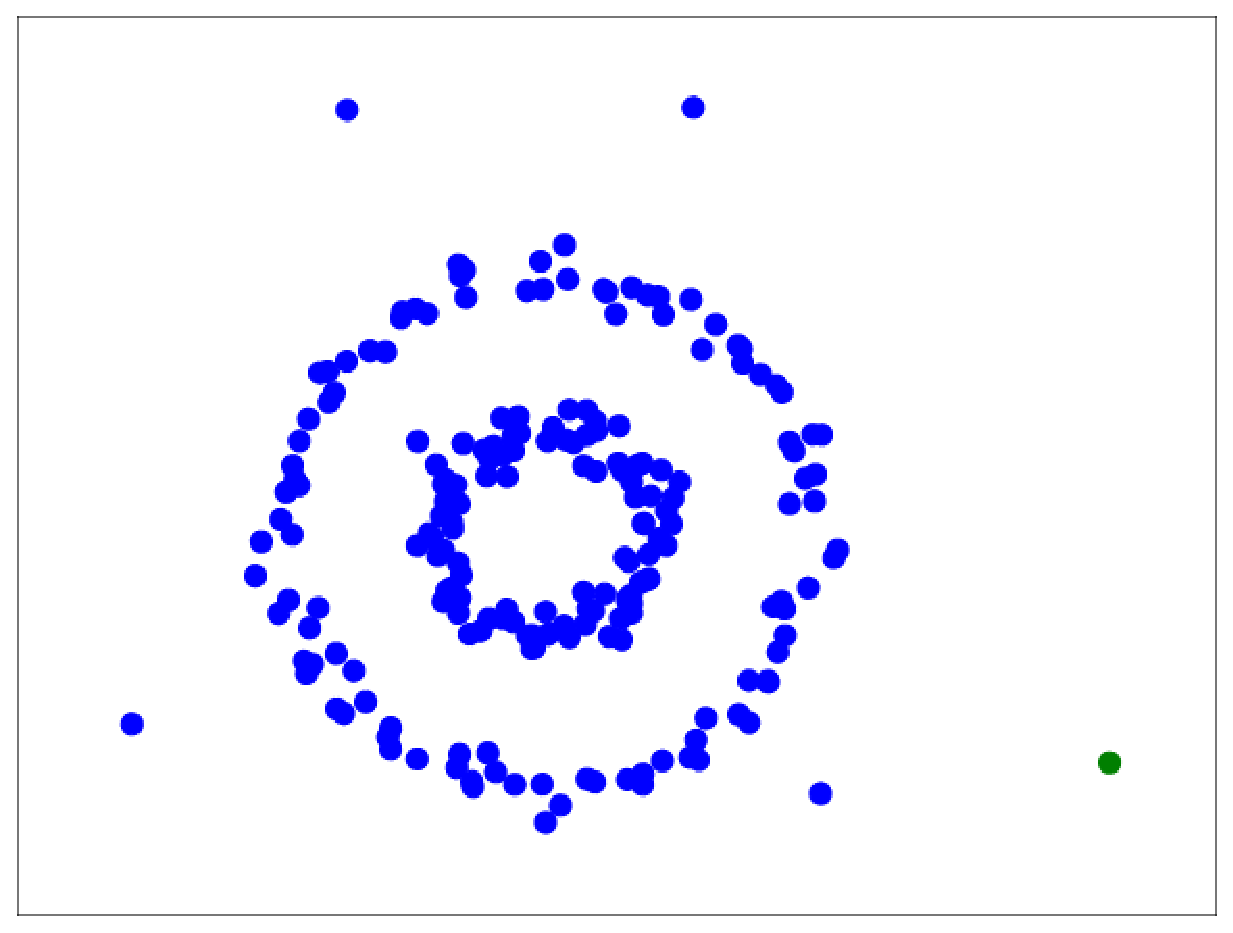
\includegraphics[width=.24\textwidth]{qualitative_circles_aggl}
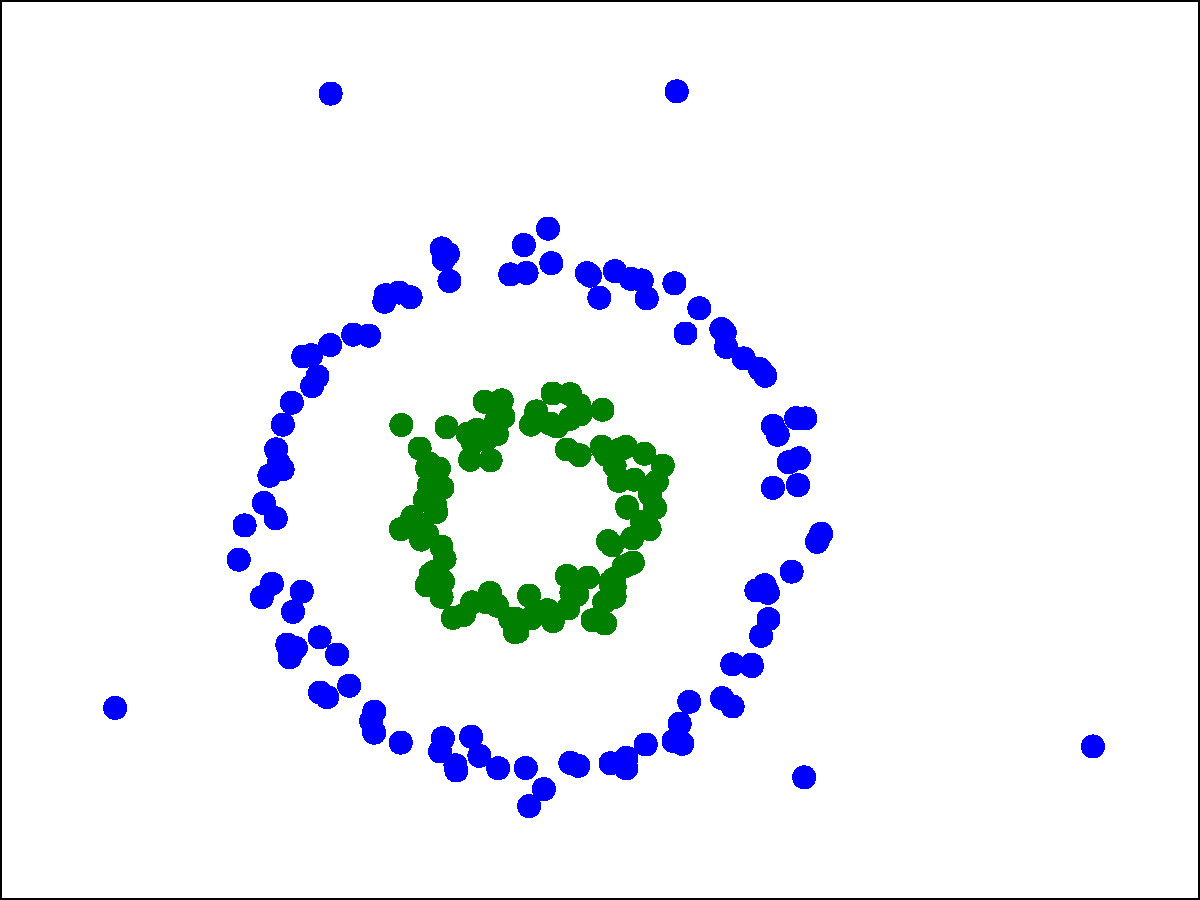
\includegraphics[width=.24\textwidth]{qualitative_circles_mst} \\ 

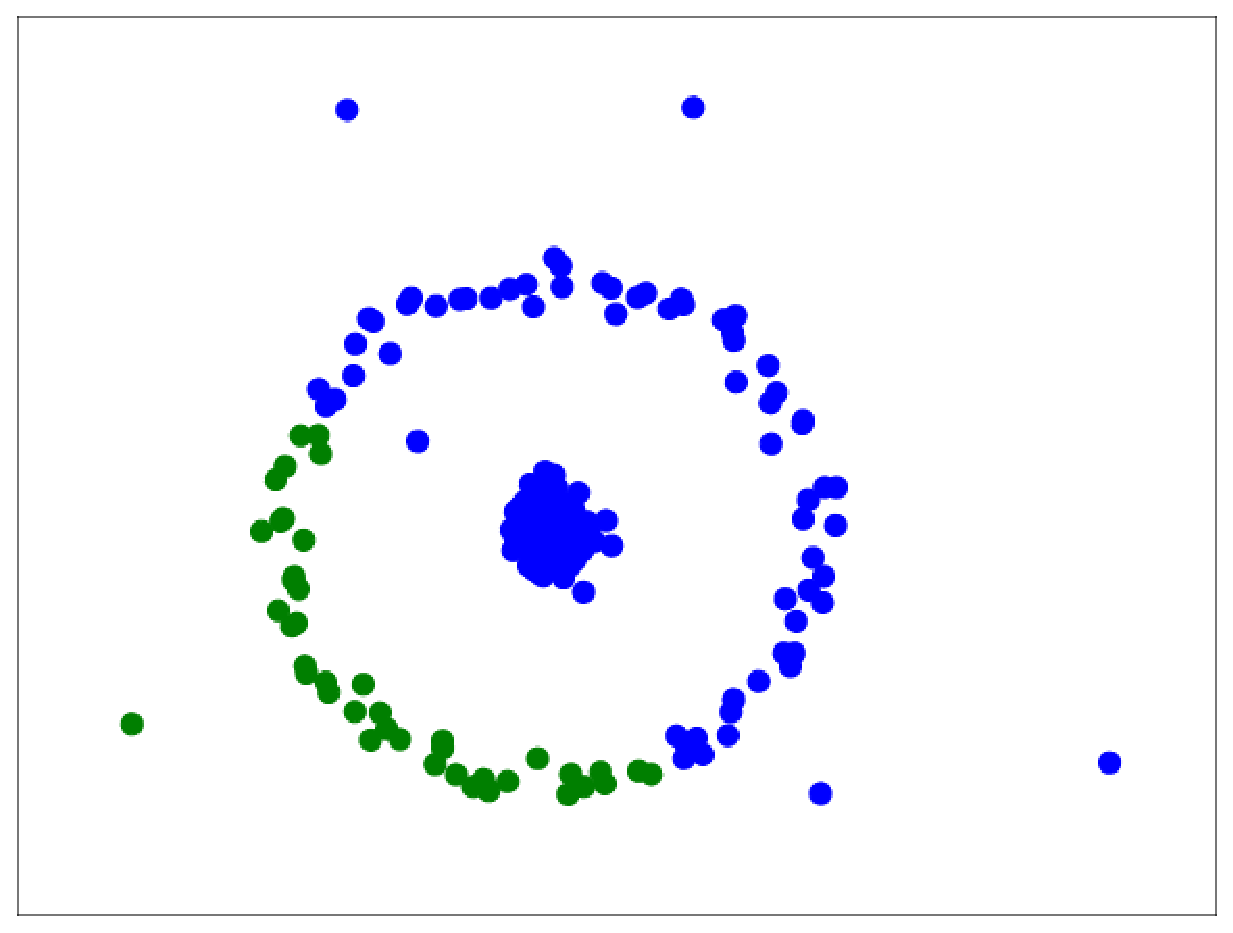
\includegraphics[width=.24\textwidth]{qualitative_circles2_km}
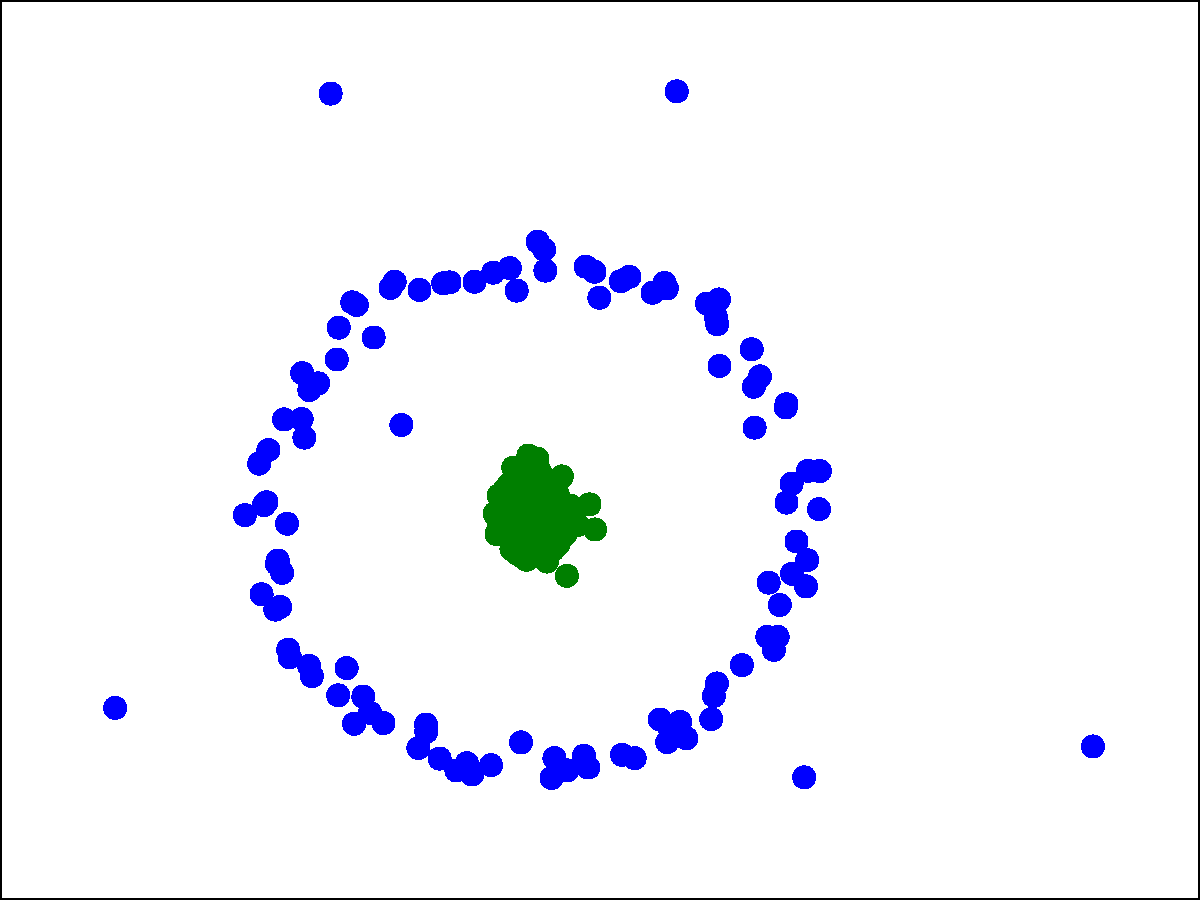
\includegraphics[width=.24\textwidth]{qualitative_circles2_mean_nn}
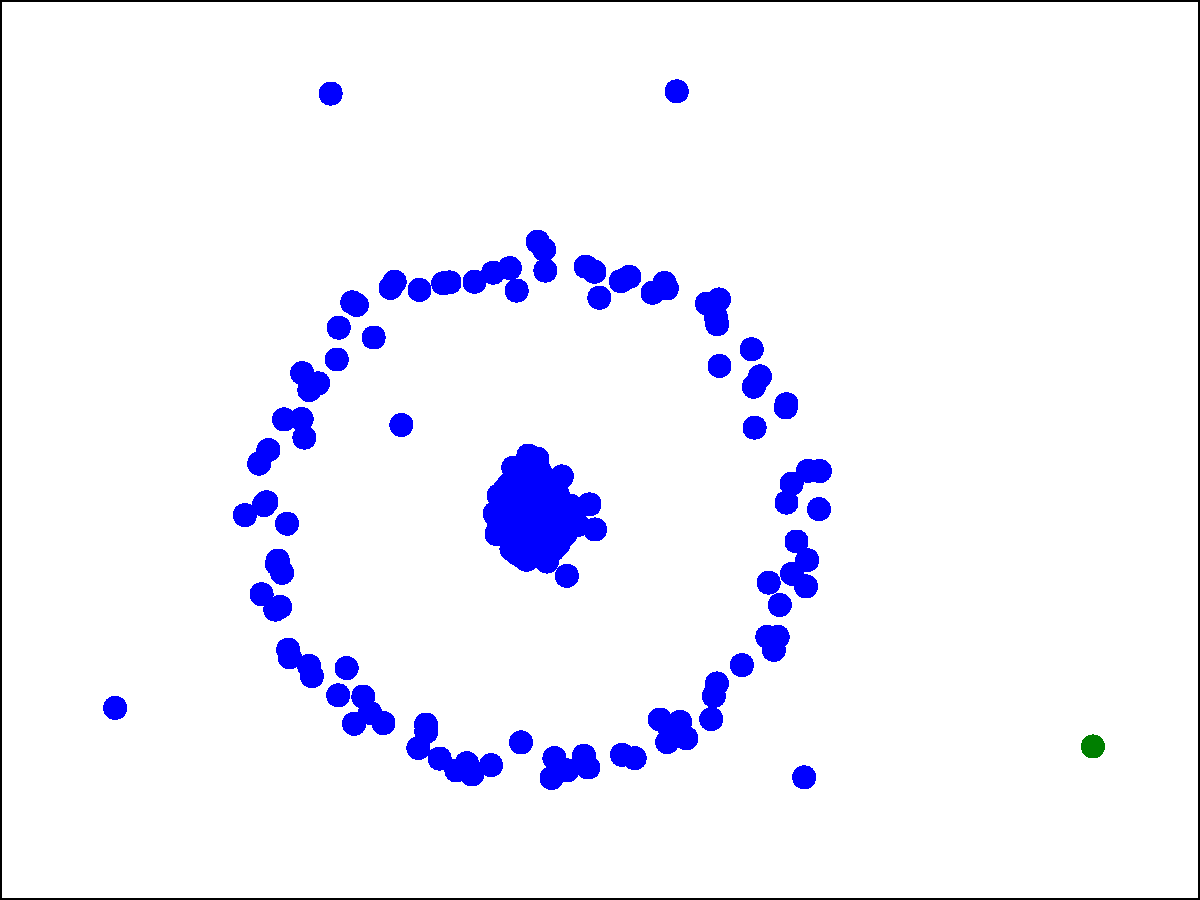
\includegraphics[width=.24\textwidth]{qualitative_circles2_aggl}
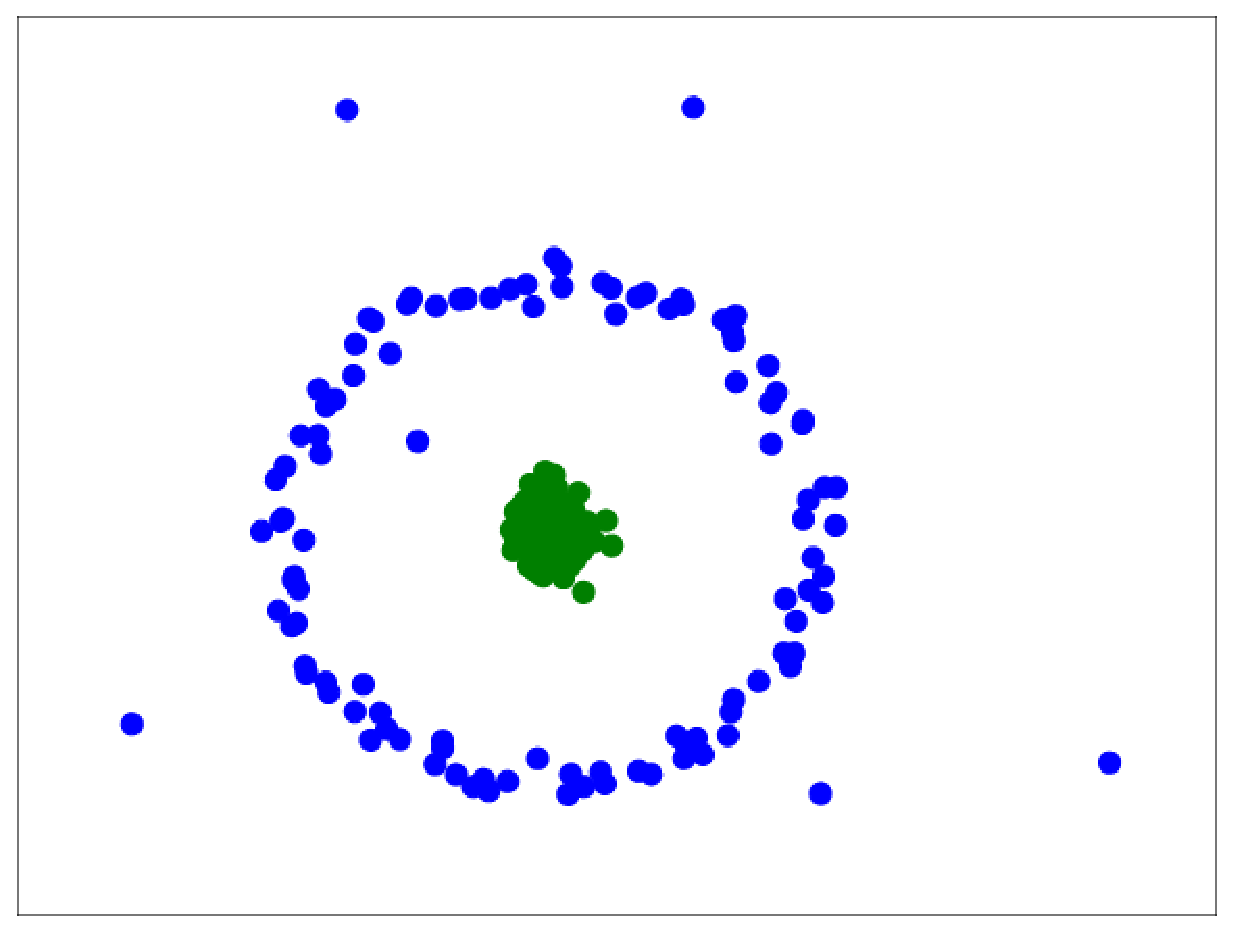
\includegraphics[width=.24\textwidth]{qualitative_circles2_mst} \\ 

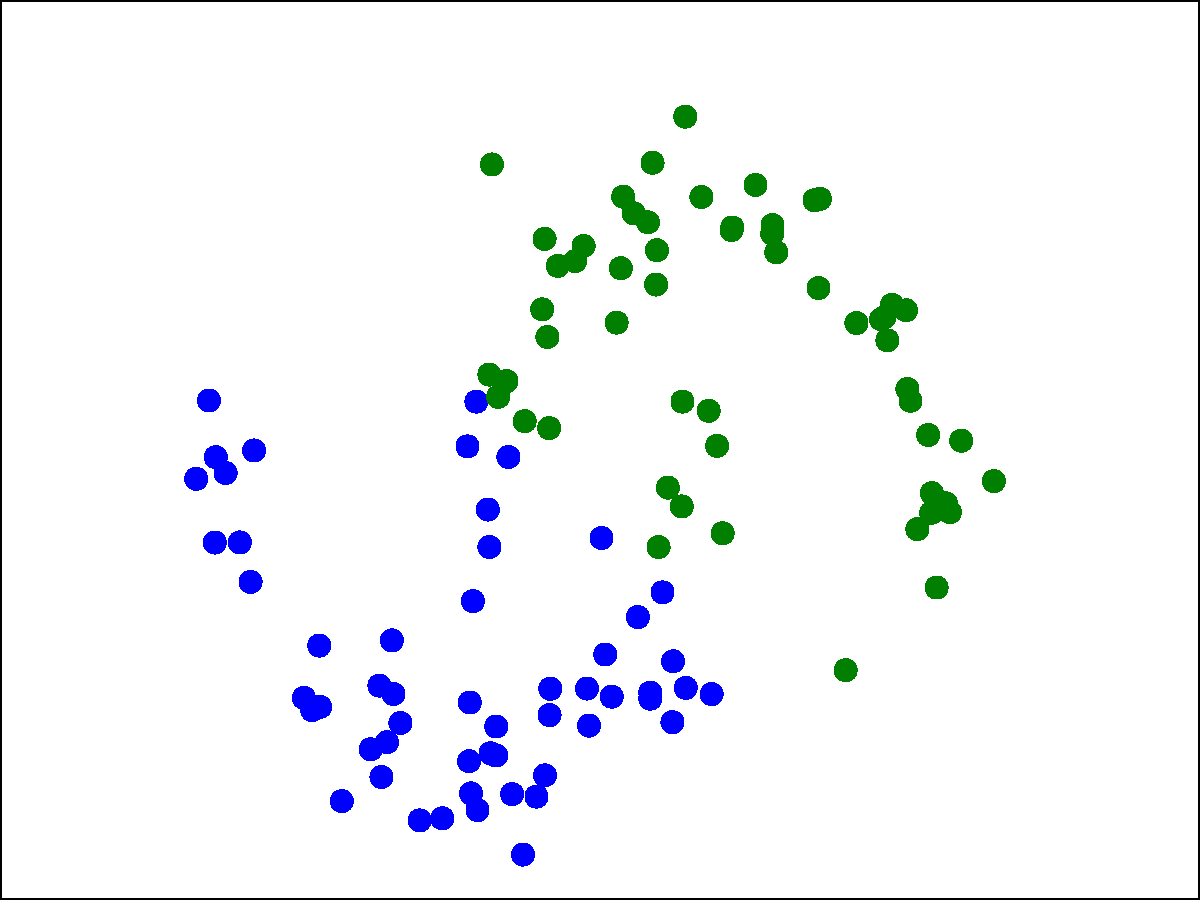
\includegraphics[width=.24\textwidth]{qualitative_twomoons_km}
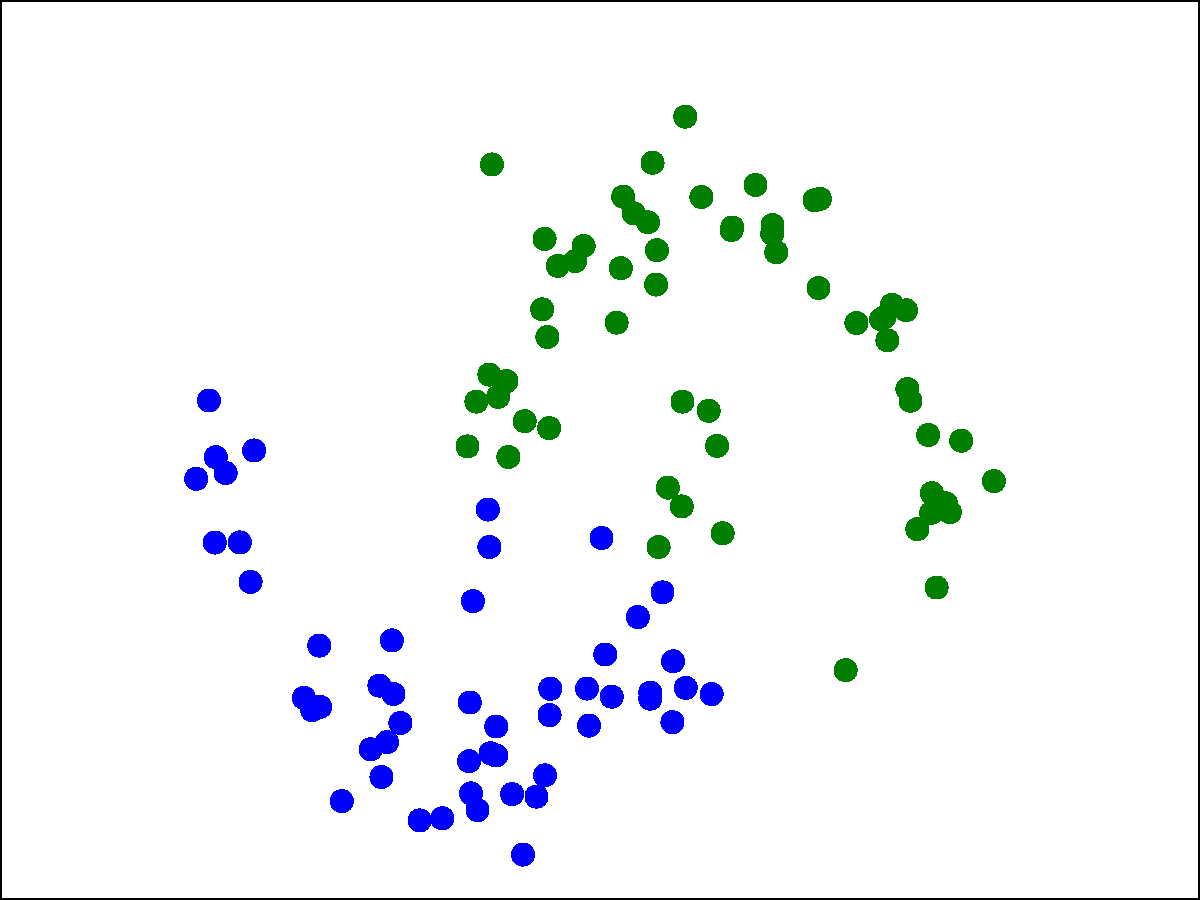
\includegraphics[width=.24\textwidth]{qualitative_twomoons_mean_nn}
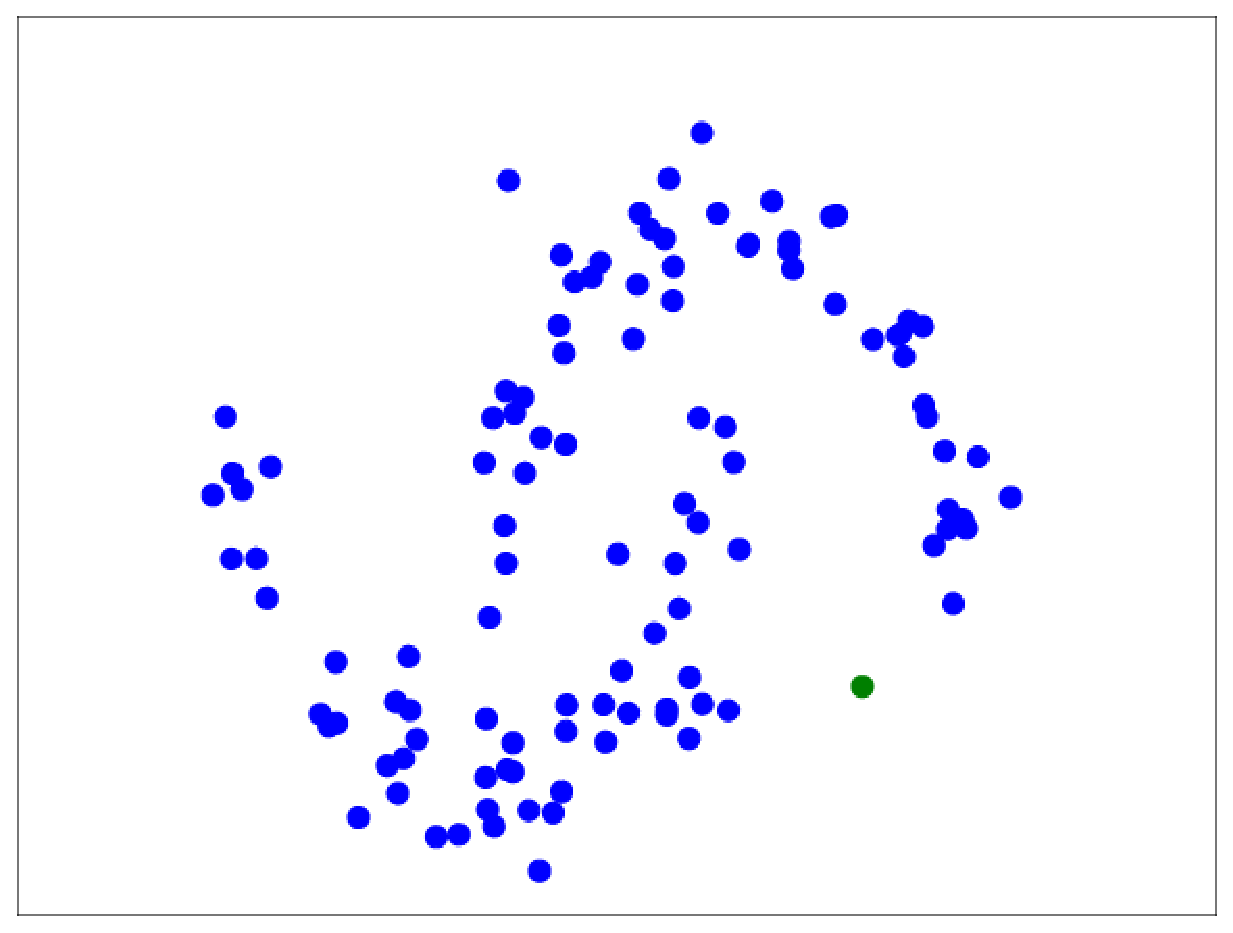
\includegraphics[width=.24\textwidth]{qualitative_twomoons_aggl}
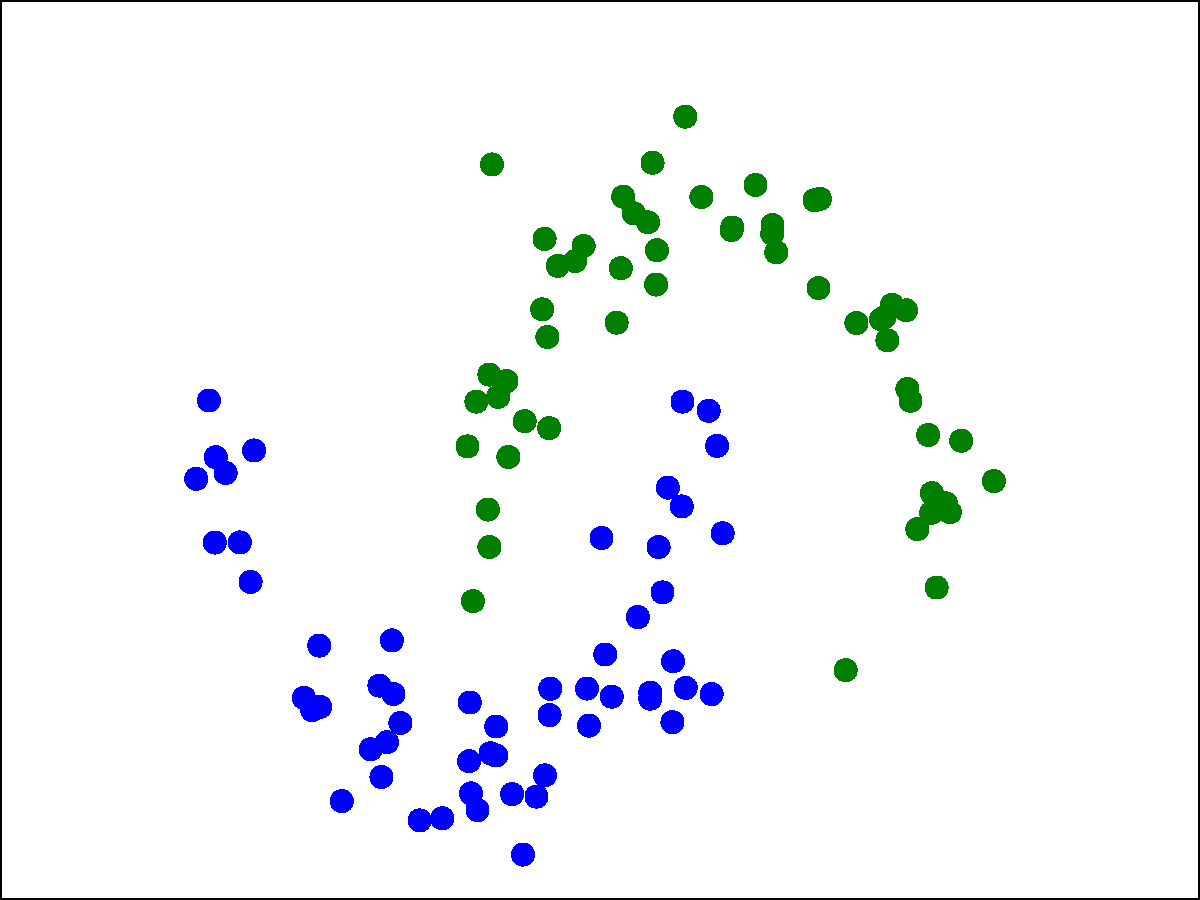
\includegraphics[width=.24\textwidth]{qualitative_twomoons_mst} \\ 
\caption{Comparison of $k$-Means (left), MeanNN (center left), single link
(center right) and ITM (right) on four synthetic datasets.  Without the need to
tune parameters, ITM can adjust to different cluster shapes.  MeanNN is able to
recover non-convex clusters (third row) but often produces similar results to
$k$-Means (second and last row). Single link clustering is very sensitive
to noise, as it does not take cluster size into account.}
\label{fig:qualitative}
\end{figure}

\section{Experiments}
We compared ITM to the popular $k$-Means algorithm 
\citep{macqueen1967some,lloyd1982least}, to the MeanNN algorithm of
\citet{faivishevsky2010nonparametric} and to single-link agglomerative
clustering~\citep{gower1969minimum}. The similarities between single-link
agglomerative clustering and the proposed MST-based optimization make it a 
good baseline for tree-based clustering approaches.

\enlargethispage{5mm}
A comparison of ITM, MeanNN and the baseline methods, $k$-Means and 
single link agglomerative clustering, in terms of their objective, 
optimization and complexity can be found in Table~\ref{nowotab}. 
We implemented the ITM clustering procedure as well as MeanNN in Python.  We
used the $k$-Means implementation available in the scikit-learn
library~\citep{pedregosa2011scikit}. The source
code is available online\footnote{\url{https://github.com/amueller/information-theoretic-mst}}.

\subsection{Experimental Setup}
For both $k$-Means and MeanNN, we restart the algorithm ten times using
different random initializations, keeping the result with the best objective
value. As ITM is deterministic there is no need for random restarts.  All of
the algorithms we compare work with a fixed number of clusters, which we set to
the number of classes in the dataset for all experiments.

As single link agglomerative clustering is sensitive to outliers, we set
a hard limit on the minimum number of samples per cluster of five for
the quantitative analysis.

\begin{table}[t]
\centering
\begin{tabularx}{\linewidth}{@{\extracolsep{\fill}}lccc}
\toprule
Algorithm &     Objective &     Det.&      Complexity \\
\cmidrule{1-4}
$k$-Means &     $\displaystyle \sum_y \sum_{i, y_i = y} \| x_i - \mu_y \|^2$ & No  & $O(nk)$ per iteration%
%\footnote{The worst-time complexity of the Lloyd-Algorithm is exponential~\cite{arthur2006slow}, though online algorithm are observed to converge in linear time~\cite{bottou1995convergence}.}
\\
MeanNN &    $\displaystyle \sum_y \log\left(\frac{1}{|\mathbf{x}_y|}\sum_{i,j, y_i=y_j=y} \| x_i - x_j \|^2 \right)$ & No & $O(n^2)$ per iteration\\
Single Link &   -- &    Yes    &    $O(n\log n)$\\
ITM & $\displaystyle \sum_{y=0}^k d p(y) \log(\bar{L}_y  ) + p(y) \log{p(y)}$ & Yes & $O(\alpha(n) n \log n + nk)$\\
\bottomrule
\end{tabularx}
\caption{Comparing properties of related algorithms. Det.\ stands for Deterministic}\label{nowotab}
\end{table}

%As our objective is motivated by limit properties of the entropy estimate of \Eqref{hmst},
%we expect the objective to work best in a setting with many samples. To avoid tautological
%solutions, we set a hard lower limit to the number of points in each cluster.
%This limit was set to $10$ for all experiments, independent of the number of samples and clusters.

\subsection{Qualitative Results}
\Figref{qualitative} shows qualitative results on three synthetic datasets.
For well separated, convex clusters, all four algorithms produce the same
clustering (see top row).  If the structure of the data is more complex, the
advantage of the proposed method is apparent.  Note that there was no need to
specify any other parameters than the number of clusters to produce these
results.  It is also noteworthy that the results of MeanNN are very close to
those produces by $k$-Means in most cases. This similarity can be explained
by the close relation of the objective functions, listed in Table~\ref{nowotab}.

\subsection{Quantitative Results}
We present results on several standard datasets from the UCI repository, 
selecting datasets that span a wide range of combinations of number
of samples, features and clusters.
To satisfy the assumption of absolute continuity of the data distribution, 
we restrict ourself to data with continuous features.

We evaluated the experiments using the \emph{adjusted Rand index 
(ARI}~\citep{hubert1985comparing}  popular measures 
of cluster quality~\citep{gomes2010discriminative,kamvar2003spectral}.
The Rand index~\citep{rand1971objective} between two clusterings counts on how
many pairs of points two clusterings agree. The adjusted Rand index contains a
calibration against chance performance.
We also measured \emph{normalized mutual information
(NMI)}~\citep{strehl2003cluster}, but do not report it here, as it resulted in
an identical ranking of the clustering algorithms.

Table~\ref{results} summarizes the results. The two entropy-based methods 
(MeanNN, ITM) have a clear advantage of the other methods, with ITM finding 
better clusterings than MeanNN in the majority of cases.
We see that ITM does well when the intrinsic dimensionality of the data matches
the feature dimension, but degraded otherwise (see ``faces'' and ``usps'').
Estimating the intrinsic dimensionality of the data overcomes this weakness,
and improves results in most cases. For all but one dataset, either ITM or ITM with
estimated intrinsic dimensionality gives the best results of all considered
algorithms.
%
The single link agglomerative clustering procedure produces reasonable 
results on datasets with little noise and well-separated clusters, but 
fails otherwise.
%
The run time of computing the ITM clustering was dominated by the computation
of the MST of the data.
%
% TODO runtime statements!
% One table datasets, one table methods + runtime?

\begin{table}[t]
\centering
\begin{tabularx}{\linewidth}{@{\extracolsep{\fill}}lrrrccccc}
\toprule
\multicolumn{4}{c}{Dataset} &\multicolumn{4}{c}{Results}\\
\cmidrule{1-4}
\cmidrule{5-9}
Description &     n &    d &   k &  $k$-Means      & MeanNN        & SL            &   ITM        & ITM ID \\
\cmidrule{1-4}                   \cmidrule{5-5}    \cmidrule{6-6}  \cmidrule{7-7} \cmidrule{8-8} \cmidrule{9-9}
digits      &  1797 &   64 &  10 &     0.62 &      0.67            &0.10          &\B{0.85}       &0.73\\ 
faces       &   400 & 4096 &  40 &     0.41 &      0.49            &0.08          &0.02           &\B{0.54}\\ 
iris        &   150 &    4 &   3 &     0.72 &      0.75            &0.55          &\B{0.88}       &0.88\\
usps        &  9298 &  256 &  10 &     0.52 &      0.54            &0.00          &   0.44        &\B{0.64}\\ 
vehicle     &   846 &   18 &   4 &     0.10 &      0.09            &0.00          &\B{0.10}       &0.10\\
vowel       &   990 &   10 &  11 &     0.17 &      0.19            &0.00          &\B{0.20}       &0.19\\
waveform    &  5000 &   21 &   2 & \B{0.37} &      0.30            &0.00          &   0.23        &0.23\\
mnist       & 70000 &  784 &  10 &     0.37 &      N/A$^\dagger$         &0.00          &   0.50        &0.77\\
\bottomrule
\end{tabularx}
\caption{Adjusted Rand Index of $k$-Means, MeanNN, single link agglomerative
    clustering and ITM on several datasets (higher is better). ITM ID refers to
    ITM using the estimated intrinsic dimensionality. The best score for each
    dataset is printed in bold.\\$^\dagger$\footnotesize We were unable to make
    MeanNN scale to 70000 data points, as storing the whole pairwise distance
    matrix seems necessary.\label{results}}
\end{table}

% TODO more experiments: mnist
% todo segmentation unsupervised
% TODO bag of word experiment?
% report times on experiments?

\section{Summary}
In this chapter we proposed the use of a minimum spanning tree based,
non-parametric entropy estimator in information theoretic clustering, ITM\@.
Thereby we extended the work of \citet{faivishevsky2010nonparametric} to a more
flexible and efficient entropy estimate.  We proposed an approximate optimization
method by formulating the clustering problem as a search over graphs.
The resulting algorithm is deterministic and has sub-quadratic run time.
%
Empirical comparisons showed that the proposed method outperforms standard
algorithms and the non-parametric entropy based clustering of
\citep{faivishevsky2010nonparametric} on multiple benchmark datasets. We
demonstrated that ITM is able to detect non-convex clusters,
even in the presence of noise.
%
In contrast to other algorithms that can handle non-convex clusters, ITM has no
tuning parameters, as the objective presents a natural trade-off between
balancing cluster sizes and enforcing intra-cluster similarity.
%
A limitation of the proposed algorithm is that it is based on the assumption 
of an absolute continuous data distribution. We show that this limitation can
be overcome in practice by estimating the intrinsic dimensionality of the data. 
%
%In future work we plan to investigate a way to overcome this limitation, 
%for example by estimating the intrinsic dimensionality of the 
%data~\citep{pettis1979intrinsic}.
%
%We also investigate optimizations of the objective 
%\Eqref{graphobjective} that go beyond the proposed method. 
%Move-making algorithms seem a promising way to refine solutions 
%found by Algorithm~1. Branch and bound techniques could provide 
%an alternative approach. 
